\documentclass[tikz]{standalone}

\usetikzlibrary{decorations.pathreplacing,shapes.multipart}

\usepackage{amssymb}

\makeatletter
\DeclareRobustCommand{\rvdots}{%
	\vbox{
		\baselineskip4\p@\lineskiplimit\z@
		\kern-\p@
		\hbox{.}\hbox{.}\hbox{.}
}}
\makeatother

\begin{document}

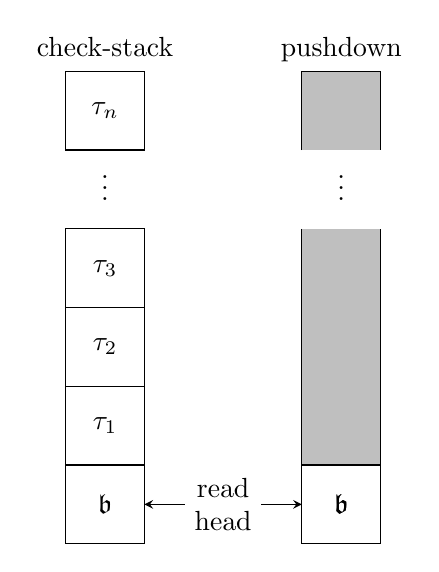
\begin{tikzpicture}[>=stealth,every text node part/.style={align=center}]

%%%%%%%%%%%%%%%%%%%%%%%%%%%%%%%%%%%%%%

\draw [draw=none,fill=none] (0,3) rectangle node {$\rvdots$} +(1,1);

\draw [fill=none] (0,-1) rectangle node {$\mathfrak{b}$}  +(1,1);
\draw [fill=none] (3,-1) rectangle node {$\mathfrak{b}$}  +(1,1);

\draw [fill=none] (0,0) rectangle node {$\tau_1$}  +(1,1);
\draw [fill=none] (0,1) rectangle node {$\tau_2$} +(1,1);
\draw [fill=none] (0,2) rectangle node {$\tau_3$} +(1,1);
\draw [fill=none] (0,4) rectangle node {$\tau_{n}$}  +(1,1);
\draw (0,5) to node[above]{check-stack\vphantom{pushdowncheck-stack}} +(1,0);


%%%%%%%%%%%%%%%%%%%%%%%%%%%%%%%%%%%%%%

\draw [draw=none,fill=none] (3,3) rectangle node {$\rvdots$} +(1,1);

\draw [fill=none] (3,-1) rectangle node {$\mathfrak{b}$}  +(1,1);
\draw [draw=none,fill=lightgray] (3,0) rectangle +(1,3);
\draw [draw=none,fill=lightgray] (3,4) rectangle +(1,1);


\draw (3,3) -- (3,0) -- (4,0) -- (4,3);
\draw (3,4) -- (3,5) -- (4,5) -- (4,4);

\draw (3,5) to node[above] {pushdown\vphantom{pushdowncheck-stack}} +(1,0);

%%%%%%%%%%%%%%%%%%%%%%%%%%%%%%%%%%%%%%

\node(rh) at (2,-0.5) {read\\head};
\draw[->] (rh) -- +(-1,0);
\draw[->] (rh) -- +(1,0);

\end{tikzpicture}
\end{document}
